%\section{Introduction}
\begin{frame}{Expectations from Midsurface Algorithm}
\begin{itemize}[noitemsep,label=\textbullet,topsep=2pt,parsep=2pt,partopsep=2pt]
\item Major impediment is the lack of precise definition \cite{Ramanathan2004}
\item Needs connectivity (no gaps) and follow the base part.
\item Existing commercial packages fail in cases of complex parts %\cite{Automex,Stolt2006a, Robinson2006,Woo2013,Lockett2008}
\item Typical failures are: 
	\begin{itemize}[noitemsep,label=\textbullet,topsep=2pt,parsep=2pt,partopsep=2pt]
	\item missing midsurface patches, gaps, overlaps
	\item not lying midway and mimicking the parent shape
\end{itemize}
\item Correcting the errors is mostly a manual, time-consuming process, requiring several hours to days. 
\item This correction time can be nearly equivalent to the time it can take to create a midsurface manually \cite{Stolt2006}. 
\end{itemize}
\begin{center}
\includegraphics[width=0.5\linewidth]{../Common/images/MidsurfaceGaps}
\end{center}
\end{frame}


\begin{frame}{Existing Methods}
\begin{itemize}[noitemsep,label=\textbullet,topsep=2pt,parsep=2pt,partopsep=2pt]
\item Some of the prominent methods: Thinning, Chordal Axis Transform (CAT), Medial Axis Transform (MAT), and Midsurface Abstraction (MA).
\item MAT and MA widely used. Commercial packages are based on MA.
\begin{figure}[h!]
\centering     %%% not \center
\subfloat[Shape]{\label{fig_tshape}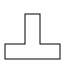
\includegraphics[width=0.3\linewidth]{../Common/images/T_part.pdf}}
\subfloat[MAT]{\label{fig_tmat}\includegraphics[width=0.3\linewidth]{../Common/images/T_mat.pdf}}
\subfloat[MA]{\label{fig_tma}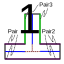
\includegraphics[width=0.3\linewidth]{../Common/images/T_ma.pdf}}
\caption{Midsurface Computation Methods}
\end{figure}
\end{itemize}
\end{frame}

\begin{frame}{Existing Methods - Problems}
\begin{itemize}[noitemsep,label=\textbullet,topsep=2pt,parsep=2pt,partopsep=2pt]
\item Midsurface is a variation of MAT, follows the parent shape completely and is devoid of extra branches \cite{Ramanathan2004}.
\item  In MA opposite faces are detected by ray casting to form the face pairs.  Each face-pair computes the  midsurface patch, which are then ``sewed'' based  on  the  adjacency  graphs.
\item Problems:
	\begin{itemize}[noitemsep,label=\textbullet,topsep=2pt,parsep=2pt,partopsep=2pt]
	\item detection of face pairs: multiple faces in front of each other, with varying degrees of overlaps, different thicknesses, etc.
	\item interaction between the face pairs: not formulated properly, then appropriate extensions, trimming and joining does not happen
	\end{itemize}
\item This work proposes to address both the problems i.e. face pair detection and interaction detection.	
\end{itemize}
\end{frame}
